In a world where the electronic technology is growing up faster than every other technology, and where portable devices are strongly common used by people, it is possible to be impressed by a new designed device. Looking to the science fictions, such as \textit{Star Trek}, it was predictable that sooner or later wearable computing is going to be part of everyday life, and so it is happening. Further, this seems to be the next step of the process in how we use computers (Fig.\ref{Fig:grow}), going from desktop usable in a fixed location only, to portability of laptops usable and connected everywhere thank to the wireless connectivity, passing to smartphones and tablets which offer a more portability, to finally wearables computing that, for the time being, offer the highest portability \cite{DDGG}.


\begin{figure}[h]
	\centering
	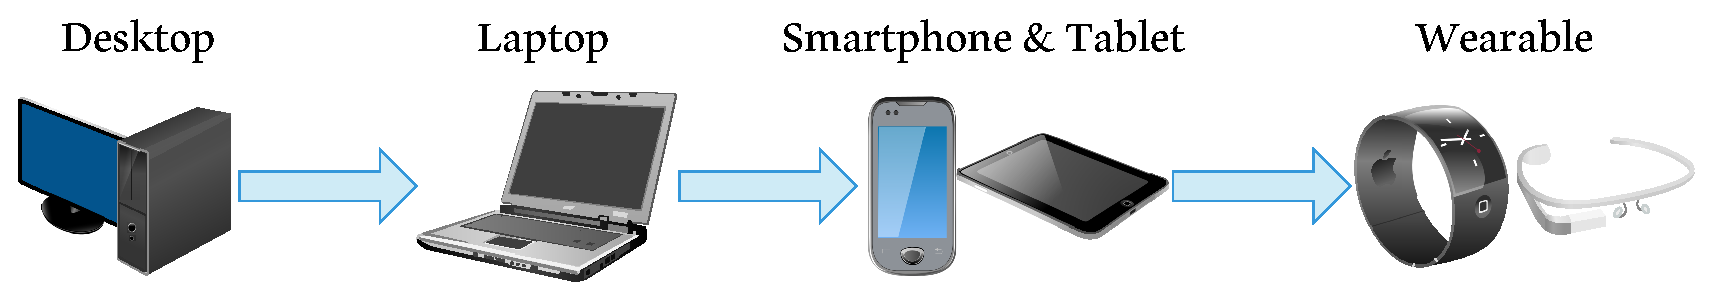
\includegraphics[width=\textwidth]{GoogleGlass/grow}
	\caption{Computing Evolution}
	\label{Fig:grow}
	
\end{figure}

Thus, \textit{smartglasses} represent an emerging space and not only Google is trying to exploit it but also other famous company like Microsoft and Sony.

\section{Google Glass}

The Google Glass hardware is listed in (Fig.\ref{Fig:glasshw}), and we can find almost all the technology installed in a smartphone, in fact Glass is made with: a battery, a micro-USB port which has the multiple functions of power source, headphone connector, and data port, a bone conduction transducer audio (\textit{BCT}) speaker, a touchpad, different sensors such as the accelerometer and gyroscope to detect head movements, WiFi and Bluetooth interface module, a camera, a microphone, and a prism which acts as display.

Google Glass is not an immersive experience, but it is on only when the user wants it, by watching on the top right corner, where the $640\ x\ 360$ display is placed, and says "\textit{Ok Google}" or tapping onto touchpad.

The Google Glass applications are called \textit{\textbf{Glassware}} and they are available in two different way: Google Mirror API and Glass Development Kit (\textit{GDK}).

\begin{figure}[h]
	\centering
	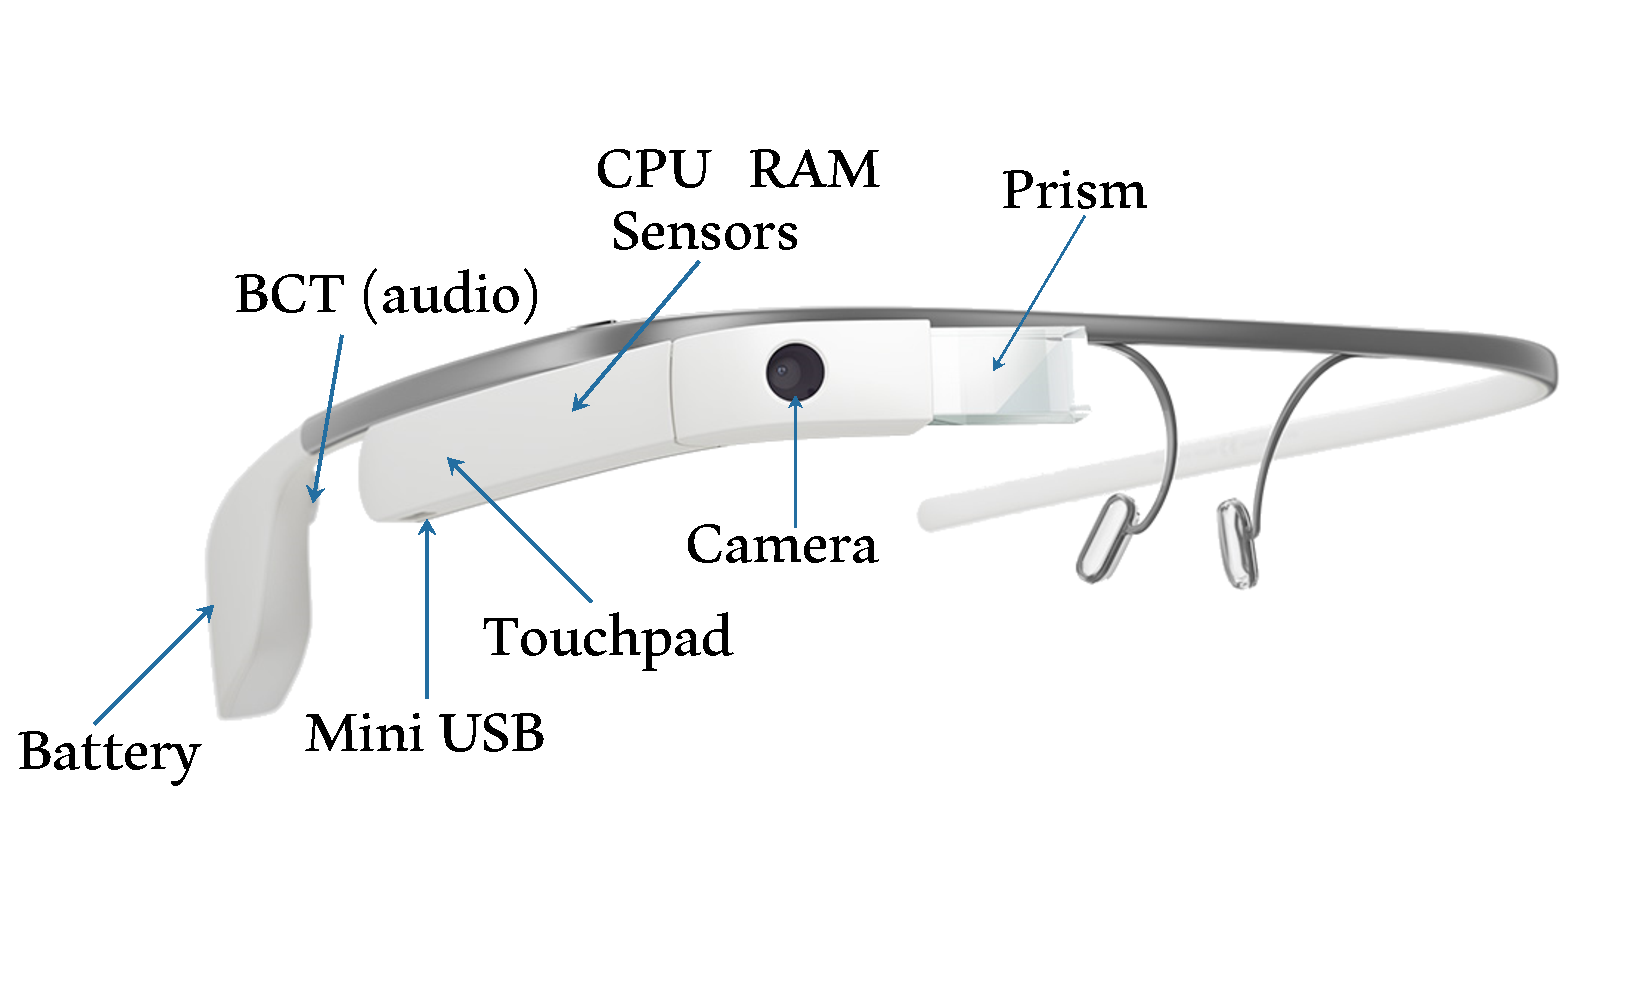
\includegraphics[width=\textwidth]{GoogleGlass/Hardware.eps}
	\caption{Google Glass}
	\label{Fig:glasshw}
\end{figure}

The \textit{timeline} is a chronological list of cards, each card represents a Glassware, does not matter which kind of it is.
In other words, timeline is a wy to organize the opened application, and users scrolling through different section of the timeline is able to reveal cards in the past, present, and future.

\subsection{Mirror API}

Mirror API Glassware is a web-based application. In fact, the code does not run on the Google Glass itself, but it runs purery in the cloud provided by Google. In this way many programming language are available: Java, Python, PHP, Ruby, .NET and Go.

The main advantage of this applications is that, because the Glassware does not run on Glass, its processor is left free to work on other things and it is not in charge to make some data manipulation, calculation and so on.. 

This service have two big requirements:  of course, being connecting and cloud-aware. Mirror API Glassware has not executable file, and has no access to the Glass sensors.

\subsection{Glass Development Kit}

Glassware built using the Glass Development Kit offers more granular control of application. The programming language available is only one: Java.

This may be defined the classic Android way, where Java code is built in an \textit{APK} (Android Package) file and installed inside the Glass device.

GDK based Glassware has more functionally tha the Mirror API one, indeed it may directly access the hardware, ensure real-time interactions, and being able offline.

The Glassware designed in this thesis is GDK based.

\chapter{The Glassware}

\begin{figure}[h]
	\centering
	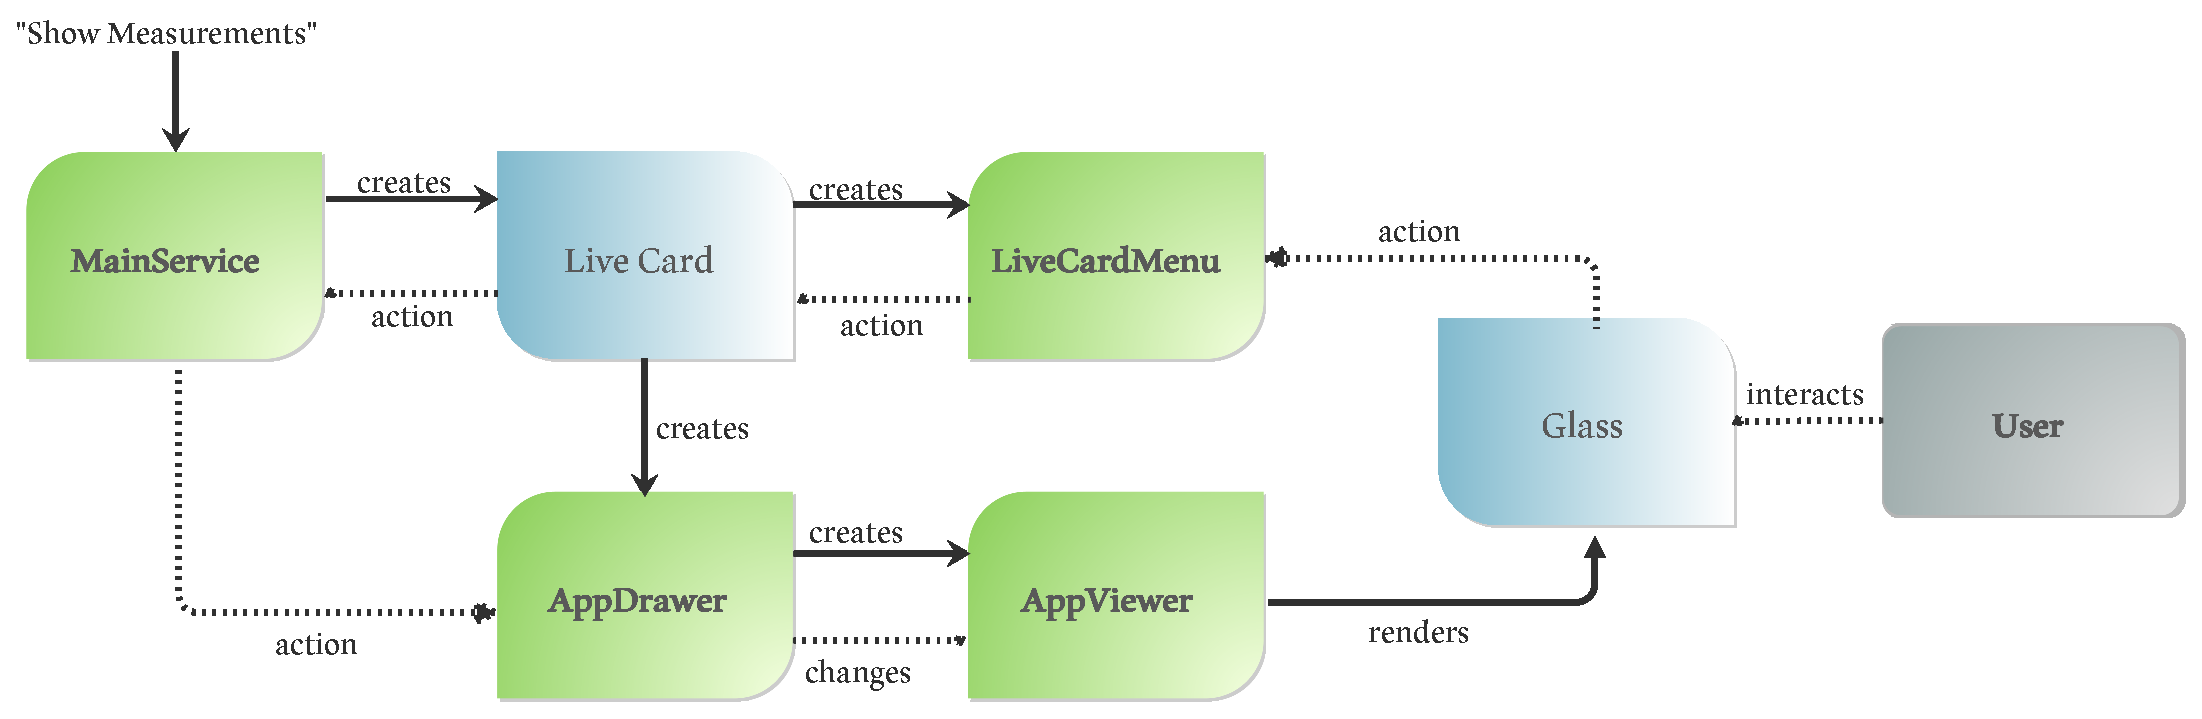
\includegraphics[width=\textwidth]{GoogleGlass/interactions}
	\caption{Interactions Between Class}
	\label{Fig:interaction}
\end{figure}

In (Fig.\ref{Fig:interaction}) how the classes and actors in the designed Glassware interact from each others is shown. This is also how a typical \textit{GDK} based Glassware works.



\begin{figure}[b]
	\centering
	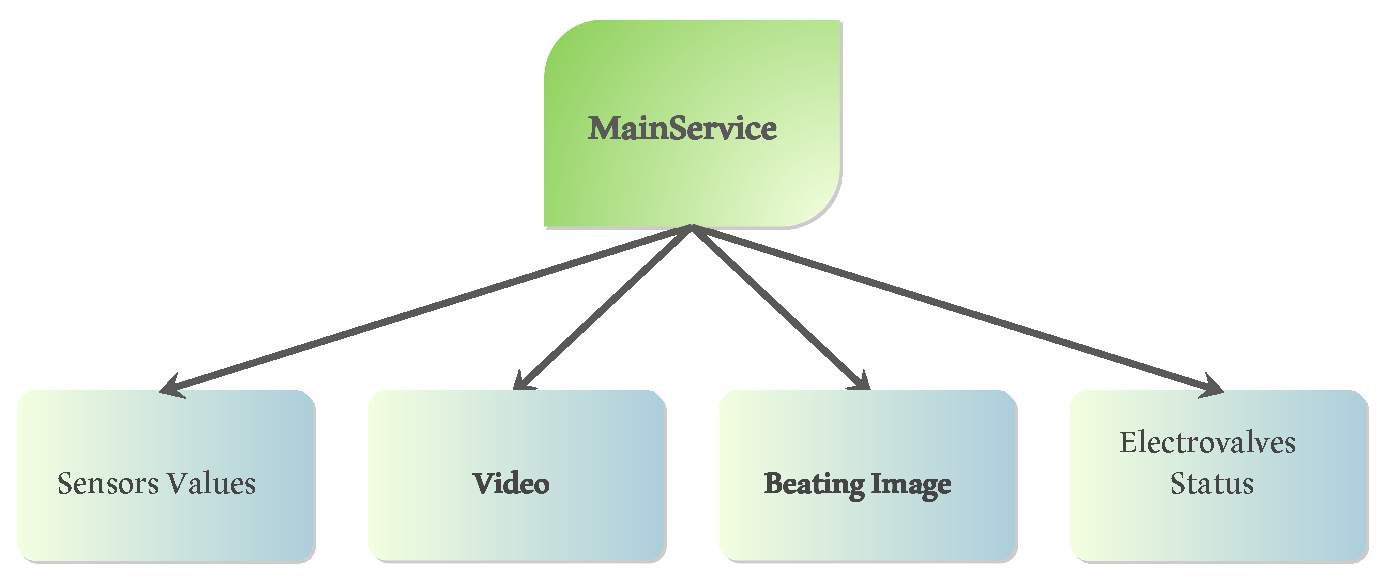
\includegraphics[scale =.5]{GoogleGlass/main}
	\caption{MainService's Runnable in Background}
	\label{Fig:mainrun}
\end{figure}

It stars with the service called \textit{MainService} (List.\ref{code:MainService}) that runs when the Glassware voice command is triggered or the application is tapped from the Google Glass Glassware list. When the service has been started, first it creates a live card and then it runs four runnable in background, (Fig.\ref{Fig:mainrun}):
\begin{itemize}
	\item \textit{Sensors Values}, a runnable that periodically downloads and updates the pH and temperature sensors values which then will be plotted.
	\item \textit{Video}, a runnable that periodically checks if a new microscope video is available and, if so, downloads this video inside the Google Glass replacing the older one.
	\item \textit{Beating Image}, a runnable that periodically downloads the beating plot replacing the older one.
	\item \textit{Electrovalves Status}, a runnable that periodically downloads the status of each valve.
\end{itemize}

A \textit{live card} is one of the most important element in the \textit{Google Glass User Interface} (\textit{UI}), it appears in the present section of the timeline and shows information that is relevant at the current time. Live cards can access low level Glass hardware, such as camera, sensors, communication modules, and so on... 

A live card persists in the present section of the timeline as long as the user thinks it may be relevant. Indeed, it is not persistent in the timeline and user can explicitly remove it through a swipe down on the touchpad. Further, more than one live cards may run at the same time, in this case, a live card is still running even if not visible and the focus is on another one.

Live cards are divided in two categories:
\begin{enumerate}
	\item \textit{Low-Frequency Rendering}, limited to a small set of views and can only update the display once every few seconds.
	\item \textit{High-Frequency Rendering}, involve content that is update frequently, more time in a second. This is very useful for plotting data coming from sensors, exactly like the application in which this Glassware is involved, this is why this kind of live card had been used in this thesis project. To create this type of live card an inflating layout has been used.
\end{enumerate}

Finally, live cards exist as long as the Android service which statically generated it is running.

\begin{figure}[h]
	\centering
	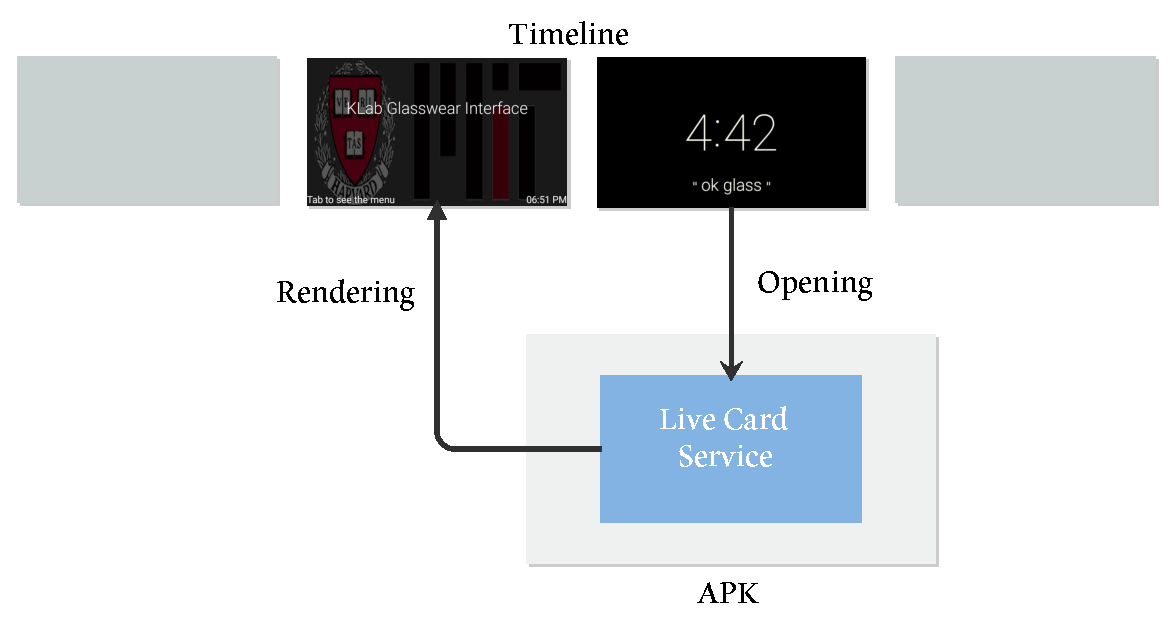
\includegraphics[width=\textwidth]{GoogleGlass/Livecard}
	\caption{Live Card, Adding to the Timeline}
	\label{Fig:livecard}
\end{figure}

Backing to the Glassware architecture, once the live card has been created, it constructs an instance of the class \textit{AppDrawer}, an implementation of \textit{Callback} for rendering and thus managing the Glassware \textit{UI}. Live card also adds an instance of the \textit{LiveCardMenu} class, which dynamically manages the menu of the Glassware. Indeed, the application menu changes based on the actual view displayed on the live card.

Then \textit{AppDrawer} creates instances of View subclass, the number of them is four: pH plot, temperature plot, beating plot and electrovalves status. In the (Fig.\ref{Fig:interaction}), these four instance are not shown for compact reasons, instead of them a generic \textit{AppViewer} class is present.

\textit{AppViewer} performs the real rendering, setting the layout and drawing the content on that.

Always in (Fig.\ref{Fig:interaction}) with continuous lines, the steps made when the Glassware has just been opened are shown, while the dashed lines highlight the interactions, that take part when the user acts on Glass.

\section{The Classes}
Below the different classes that compose the Glassware are going to be shown.
\subsection{Main Service}

The code of the main service class is displayed in (List.\ref{code:MainService}). As already said, this class is in charge to create the live card, and to it the live time of the Glassware itself is tied. So, this happens when the service is started at the \textit{OnStartCommand}. After that, an \textit{AppDrawer} instance is created and set as callback in order to render the live card surface.

The \textit{OnStartCommand} method also creates the runnable tasks which run in background to update the data information coming from the Google App Engine Datastore

Finally the main service is also in charge to handle the user requests, that are passed through the menu activity.

\subsection{App Drawer}

The code of the App drawer is shown in (List.\ref{code:AppDrawer}). This subclass allows the control of display surface and chooses which View as to be set at a given time. In fact, it first creates an instance of each view subclass, with their \textit{listener} interface. Then implements the listener method, this is a convenient way to skip from a view to another one. Finally it runs the view draw request, locking the surface canvas.

\subsection{Menu Activity}
The code of the menu activity is shown in (List.\ref{code:MenuActivity}). This subclass plays a very relevant role in the  Glassware functionality. Indeed, it shows the different chooses that allow the user to navigate into the application.

To fulfill that aim it has to change dynamically, based on what is the viewer on focus of the live card. From the main view, user can choose one of the following options: \textit{View pH}, \textit{View Temperature}, \textit{View Video}, \textit{View Beating}, \textit{Drive Electrovalves}, and \textit{Exit}.

\begin{figure}[h]
	\centering
	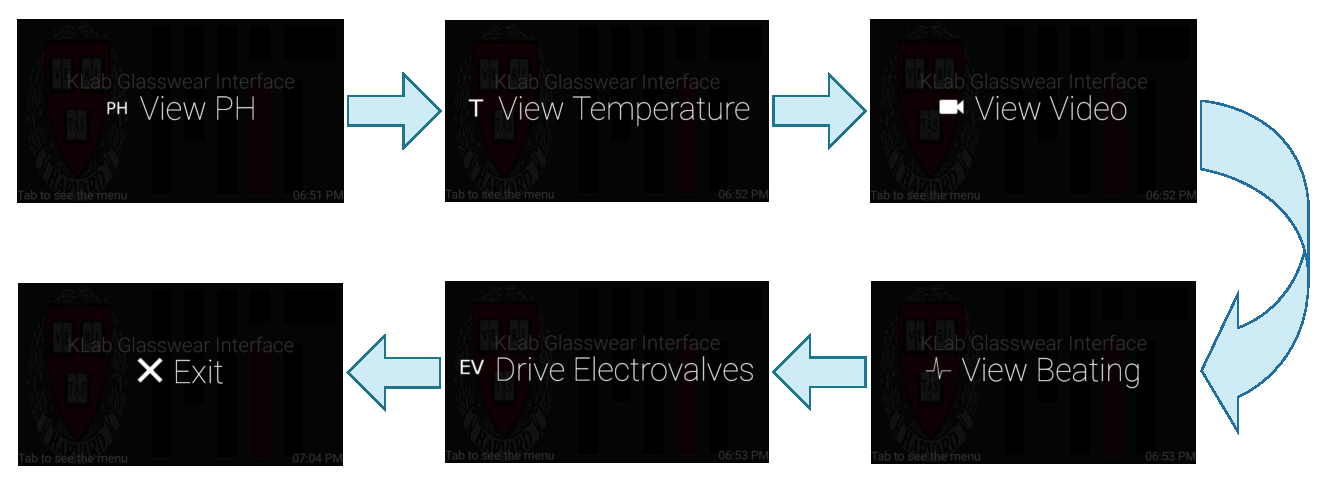
\includegraphics[width=\textwidth]{GoogleGlass/mainmenu}
	\caption{Main Menu}
	\label{Fig:mainmenu}
	\hfill
\end{figure}

To navigate the menu, user must scroll with a finger, swiping on the touchpad.

The image in (Fig.\ref{Fig:mainmenu}) shows the menu options from the Glassware main view. The (Fig.\ref{Fig:menu1}) shows the menu options when the graphs (pH, temperature, and beating) are displayed.\\
Finally, (Fig.\ref{Fig:menuev}) shows the menu options when the \textit{Drive Electrovalves} is displayed. In that figure only four choses of eight are shown, for compact reasons only. To toggle the valves the Glassware uses two classes: Electrovalves, static class where the status of the valves is stored, and HTTP subclass of Android service, used to send HTTP \textit{GET} and \textit{POST}. The parameter of the HTTP request are attached to the intent that creates the service.



\begin{figure}[h]
	\centering
	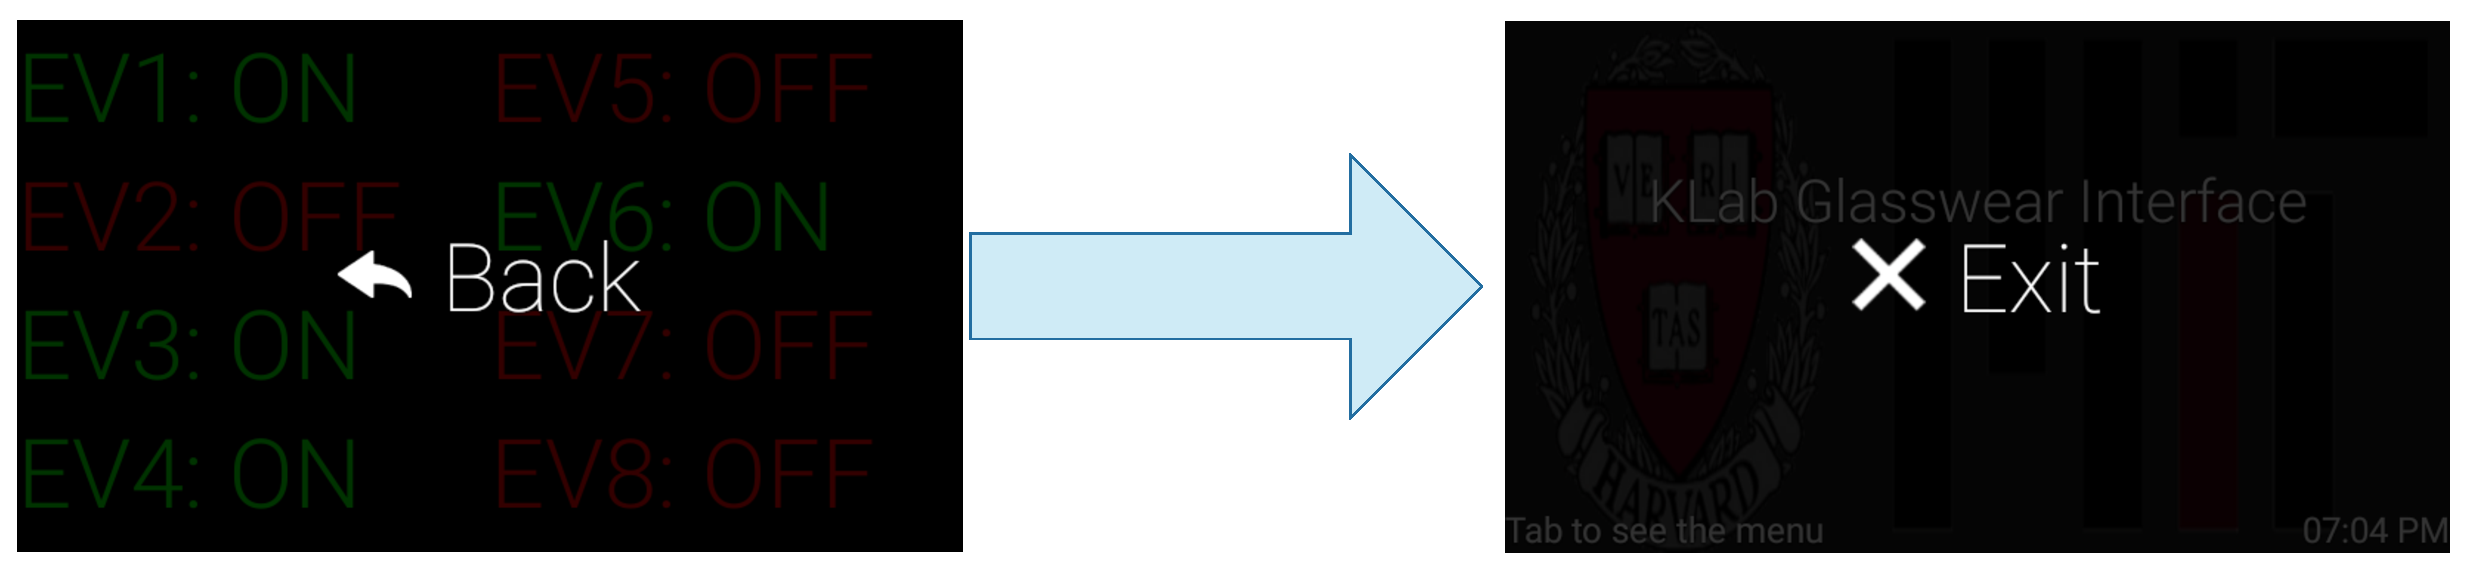
\includegraphics[width=0.75\textwidth]{GoogleGlass/menu1}
	\caption{Graph Menu}
	\label{Fig:menu1}
\end{figure}

\begin{figure}[h]
	\centering
	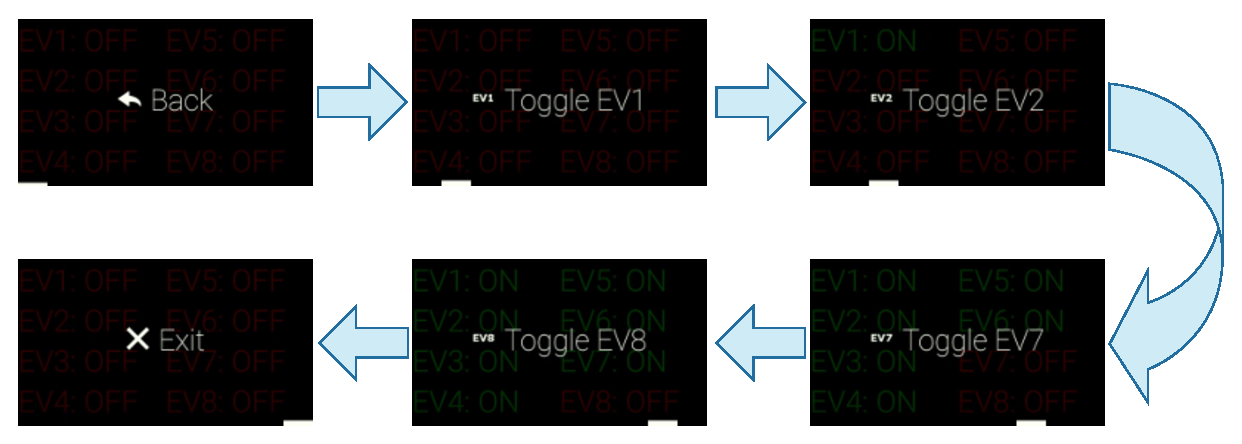
\includegraphics[width=\textwidth]{GoogleGlass/menuev}
	\caption{Menu Electrovalves}
	\label{Fig:menuev}
\end{figure}

Thus, the menu activity is in charge to show dynamically the possible options as well as handle the requests using the Android \textit{intents} to inform the other subclasses what they are supposed to do.

\subsection{App Manager}

The code of this class is shown in (List.\ref{code:AppManager}). The \textit{App Manager} is a static class that is in charge to memorize the state, what is the view that has to be displayed.

\subsection{Main View}

The code of this class is shown in (Lis.\ref{code:MainView}). The \textit{Main View} instantiates the layout \textit{XML} file and sets the Harvard-MIT logo as background image, \textit{"KLab Glassware Interface"} as main written, "Tab to see the menu" as left footer, and the current hour as right footer.
\begin{figure}[h]
	\centering
	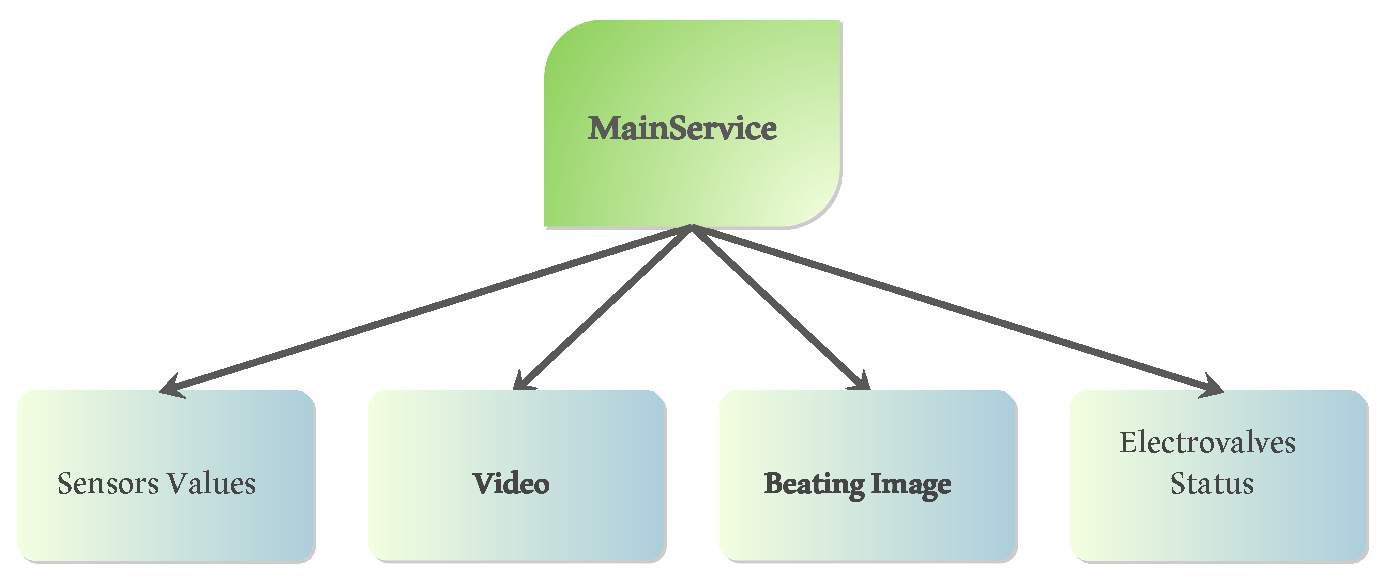
\includegraphics[width=.55\textwidth]{GoogleGlass/main}
	\caption{Main View}
	\label{Fig:main}
\end{figure}

\subsection{PH and Temperature Views}

Their codes are shown in (List.\ref{code:PHViewer}) and (List.\ref{code:TemperatureView}). As for the main view, also this subclass instantiates a layout \textit{XML} file and plot the data, write the kind of sensor is it ("\textit{Temperature}" or "\textit{pH}") on the top, and the value of the last data point on the bottom. 
\begin{figure}[h]
	\centering
	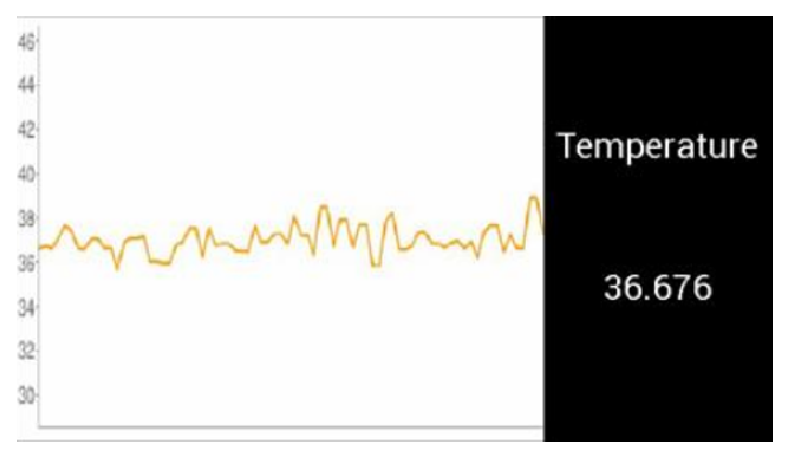
\includegraphics[width=.55\textwidth]{GoogleGlass/temperature}
	\caption{Temperature View}
	\label{Fig:temperature}
\end{figure}

\subsection{Beating View}

The last plot, the beating one, is shown in (Fig.\ref{Fig:beating}). The code of this subclass is listed in (List.\ref{code:BeatingView}). In this case the layout is made by an \textit{ImageView} only, and the subclass just set the stored beating plot image.

\begin{figure}[h]
	\centering
	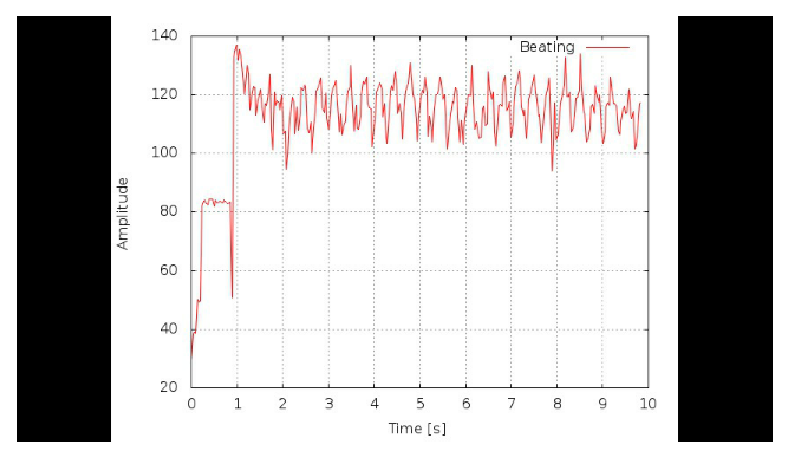
\includegraphics[width=.55\textwidth]{GoogleGlass/beating}
	\caption{Beating View}
	\label{Fig:beating}
\end{figure}

\subsection{Electrovalves View}

\begin{figure}[h]
	\centering
	\subfloat[When Status Has Not Dowloaded Yet\label{subfig-1}]{%
		\includegraphics[width=.5\textwidth]{GoogleGlass/bobo}
	}
	\subfloat[When They Are All Off\label{subfig-2}]{%
		\includegraphics[width=.5\textwidth]{GoogleGlass/electrovalves_all_off}
	}
	\hfill
	\subfloat[When Some of Them is On\label{subfig-3}]{%
		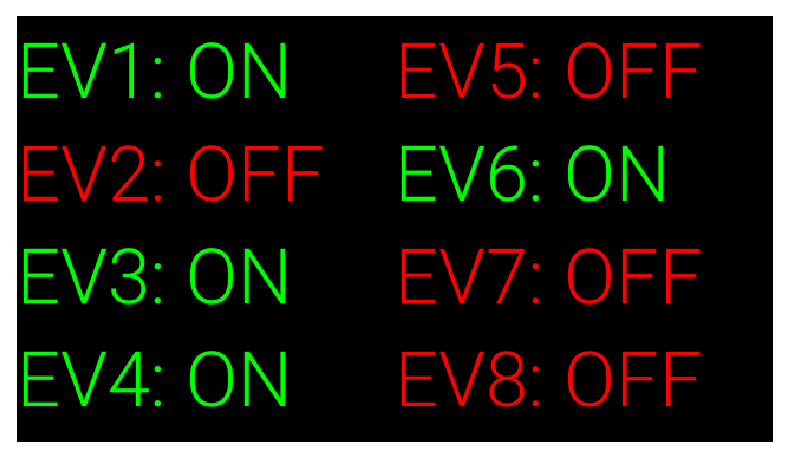
\includegraphics[width=.5\textwidth]{GoogleGlass/elecreovalves_random_status}
	}
	
	
	\caption{\textit{Electrovalves View}}
	\label{elele}
	
\end{figure}

The (Fig.\ref{elele}) shows the result of the electrovalves view. It lists all the eight valves showing the corresponding status. When the user opens the \textit{Drive Electrovalves} tab and the background tasks has not downloaded the valves status yet, the whole electrovalves are displayed without their status, and white written, (Fig.\ref{subfig-1}). When the valves status has been downloaded, the name and the status appear in green color if the valve is on, or in red if it is off, (Fig.\ref{subfig-2}) and (Fig.\ref{subfig-3}).

\subsection{Video Activity}

To play the stored video on Google Glass there are two way, the first one uses the \textit{VideoView} object, and the second one uses an intent belonging to Google Glass API: com.google.glass.action.VIDEOPLAYER. The Glassware described so far exploits this second way, because so the video player is optimized for the Google Glass. Indeed, user can navigate into the video with simple horizontal swipes on the touchpad (Fig.\ref{subfig-45}), can stop the video with a simple tap (Fig.\ref{subfig-35}), and to close the video uses a vertical swipe.

\begin{figure}[h]
	\centering
	\subfloat[Video\label{subfig-45}]{%
		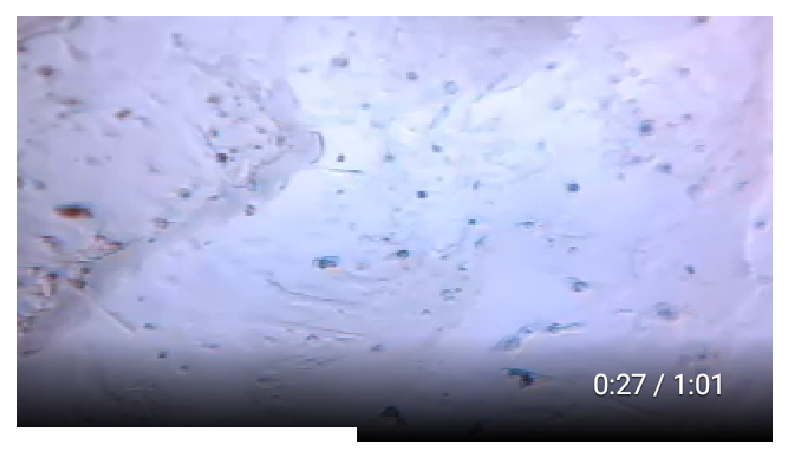
\includegraphics[width=.5\textwidth]{GoogleGlass/video}
	}
	\subfloat[Video on Pause\label{subfig-35}]{%
		\includegraphics[width=.5\textwidth]{GoogleGlass/video_pause}
	}
	
	
	\caption{\textit{Microscope Video}}
	\label{ool}
	
\end{figure}